%----------------------------------------------------------------------------------------
%	CURRICULUM VITAE
%----------------------------------------------------------------------------------------

\makecvtitle % Print the CV title

%----------------------------------------------------------------------------------------
%	EDUCATION SECTION
%----------------------------------------------------------------------------------------

\section{Education}

\cventry{2014--2016}{Master of Science - Multimodal and Cognitive Systems}{University of Zürich}{}{}{Modules included:
\begin{itemize}
	\item Fundamentals of Image Processing and Computer Vision
	\item Autonomous Mobile Robots
	\item Introduction to Machine Learning (ETH Course)
	\item Neuromorphic Engineering II
	\item Neurophysics
	\item Complex Systems: Berechenbares Chaos in dynamischen Systemen
	\item Master Project: Head Pose Tracking with Quadrotors with Headmounted camera
\end{itemize}}  % Arguments not required can be left empty

\cventry{2009--2013}{Bachelor of Science - Applied Informatics: Neuroinformatics}{University of Zürich}{}{}{Modules included:
\begin{itemize}
	\item Neuromorphic Engineering I
	\item Theory, Programming and Simulation of Neural Networks
	\item Systems Neuroscience
	\item Computational Vision
	\item Introduction to Neuroinformatics
\end{itemize}}

\cventry{2008--2009}{Passerelle}{AKAD College}{}{}{The Passerelle is an exam which, together with a Berufsmatura, qualifies as a Matura and allows studying at a University.}

\cventry{2003--2007}{Informatikmittelschule}{Kantonsschule Enge}{}{}{
The Informatikmittelschule provides a practically oriented education as a programmer and is similar to an apprenticeship. The first three years consist of programming lessions and standard school subjects with a focus on economics. Finally, there are exams and a Berufsmatura is obtained. The last year is an internship, including a two week project, which must be done at a company. My project was a prototype of a chemical monitoring system for water recycling plants.}

\cventry{1999--2003}{Gymnasium, Ancient language profile}{Kantonsschule Freudenberg}{}{}{I completed 4 years at the Gymnasium with focus on languages (German, French, Spanish, Latin). After the 4th year I decided to drop it in favour of the Informatikmittelschule because I had lost the interest in languages.}

\section{Masters Thesis}

\cvitem{Title}{\emph{Paper Tracking} - A real time algorithm}
\cvitem{Supervisor}{Prof. Dr. Chat Wacharamanotham}
\cvitem{Description}{I developed an algorithm that is capable of finding a paper inside a frame recorded by a digital camera mounted on the reader's head. It looks for areas with a high density of color intensity changes. The detected paper is matched against a database of PDFs using SURF features. In a final step it scans the PDF in the database for statistical graphics by analyzing the figures using visual words based feature vectors and an SVM with an RBF kernel.}
\cvitem{Grade}{\textbf{5.75}}

\section{Bachelor Thesis}

\cvitem{Title}{\emph{Maggie} - An Infant Robot Model}
\cvitem{Supervisor}{Dr. Hugo Gravato Marques}
\cvitem{Description}{I built a physical prototype of an infant robot model including an API to control it from a PC and collect data. It is made out of spare metal parts, servo motors, force resisting sensors, two cameras, IMUs and 3D designed and printed parts.}
\cvitem{Grade}{\textbf{5.5}}

%----------------------------------------------------------------------------------------
%	WORK EXPERIENCE SECTION
%----------------------------------------------------------------------------------------

\section{Experience}

\cventry{2012--2015}{Software Developer}{\textsc{New Voice AG}}{Zürich}{}{New Voice AG is a company located in Zürich which develops a software called MobiCall which is an Alarm-, Information-, Conference and Callrecording system which is built on top of a PBX system. My responsibility was to develop and maintain a plugin for locating Dect and WiFi devices inside buildings and triggering alarms.}

%------------------------------------------------

\cventry{2011--2012}{Software Developer}{\textsc{TrueBPM Solutions AG}}{Zürich}{}{TrueBPM develops a BPM system that is used internally by an assurance company. While I was working there, I was responsible for letter generation. I had to design BIRT reports based on word documents and also do some server backend programming. I left the company after a year, because the project was finished and I wanted to do something more challenging.}

%------------------------------------------------

\cventry{2006--2011}{Software Developer}{\textsc{IT-GR GmbH}}{Zürich}{}{IT-Gr GmbH is a software developing company. During my time there I worked alone on a monitoring system for water recycling plants for a customer called Unimon GmbH. The software periodically pulls measured data from different sensors embedded in the water plant. Users can log in through a web interface, analyze the data and create reports. It is also possible to define conditions under which alarms are  triggered. It then automatically contacts the responsible person per E-Mail or SMS.
\newline
My first year there (2006-2007) was an Internship as part of the “Informatikmittelschule”.}

%----------------------------------------------------------------------------------------

%----------------------------------------------------------------------------------------
%	REFERENCE CONTACTS SECTION
%----------------------------------------------------------------------------------------

\newpage

\section{Reference Contacts}

\subsection{Prof. Dr. Chat Wacharamanotham}
\cvitem{Link}{\href{http://www.ifi.uzh.ch/en/zpac/people/chat.html}{http://www.ifi.uzh.ch/en/zpac/people/chat.html}}
\cvitem{}{Supervision of Master Thesis}
\cvitem{E-Mail}{\href{mailto:chat@ifi.uzh.ch}{chat@ifi.uzh.ch}}
\cvitem{Phone}{+41 (0)44 635 43 13}

\subsection{Prof. Dr. Davide Scaramuzza}
\cvitem{Link}{\href{http://rpg.ifi.uzh.ch/people\_scaramuzza.html}{http://rpg.ifi.uzh.ch/people\_scaramuzza.html}}
\cvitem{}{Supervision of Master Project}
\cvitem{E-Mail}{\href{mailto:sdavide@ifi.uzh.ch}{sdavide@ifi.uzh.ch}}
\cvitem{Phone}{+41 (0)44 635 24 09}

%----------------------------------------------------------------------------------------
%	COMPUTER SKILLS SECTION
%----------------------------------------------------------------------------------------

\section{Computer skills}

\cvitem{Basic}{\textsc{Bash Scripts}, QT, Cuda}
\cvitem{Intermediate}{\textsc{java}, \textsc{html}, \textsc{JavaScript}, \LaTeX, Microsoft Windows, OpenCV, Computer Hardware, Scikit Learn}
\cvitem{Advanced}{\textsc{python}, \textsc{C++}, Linux}

%----------------------------------------------------------------------------------------
%	LANGUAGES SECTION
%----------------------------------------------------------------------------------------

\section{Languages}

\cvitemwithcomment{German}{Mothertongue}{}
\cvitemwithcomment{Spanish}{Mothertongue}{}
\cvitemwithcomment{English}{Intermediate}{Conversationally fluent}

%----------------------------------------------------------------------------------------

%----------------------------------------------------------------------------------------
%	INTERESTS SECTION
%----------------------------------------------------------------------------------------

\section{Interests}

\renewcommand{\listitemsymbol}{-~} % Changes the symbol used for lists

\cvlistdoubleitem{Reading}{Jiu Jitsu}
\cvlistdoubleitem{Karate}{Cooking}
\cvlistdoubleitem{Workout}{Swimming}

\newgeometry{bottom=0pt}
\section{Master Grades - Exempt from module booking system}
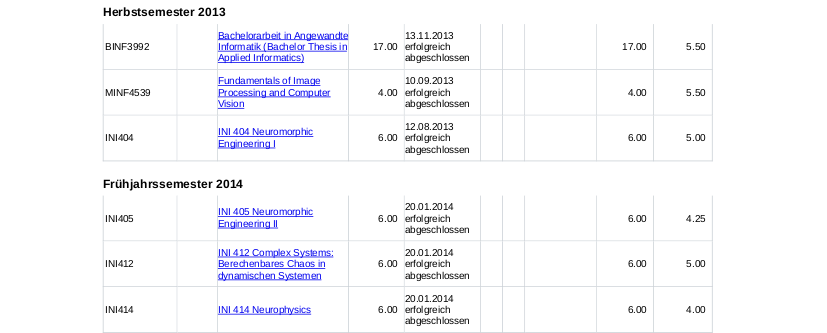
\includegraphics[width=\textwidth]{pictures/master/module1.png}
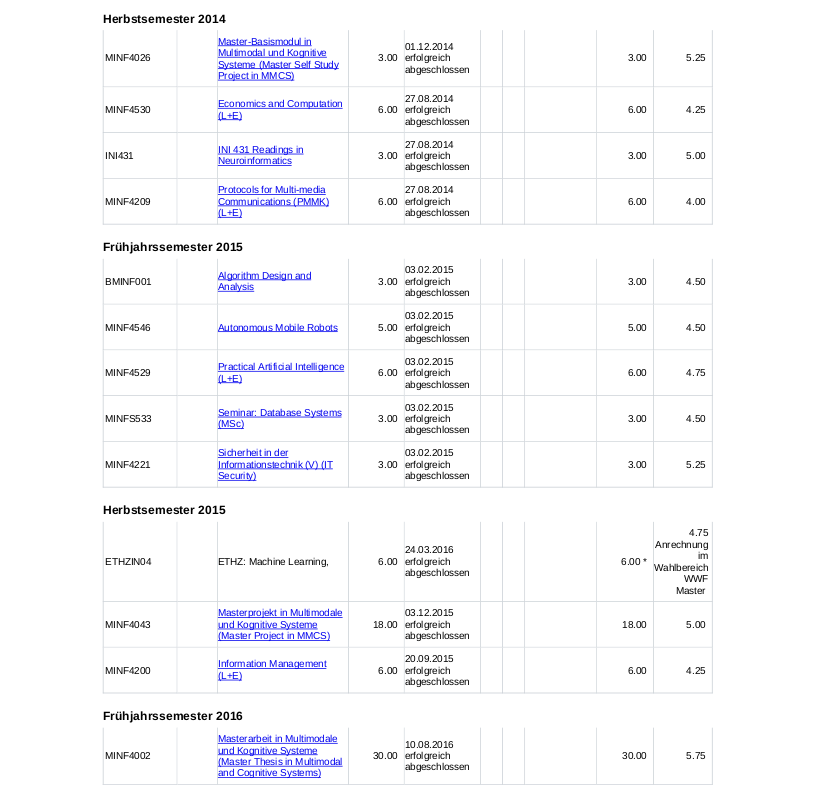
\includegraphics[width=\textwidth]{pictures/master/module2.png}

\enlargethispage{12pt}
\newpage
\section{Bachelor's Diploma}
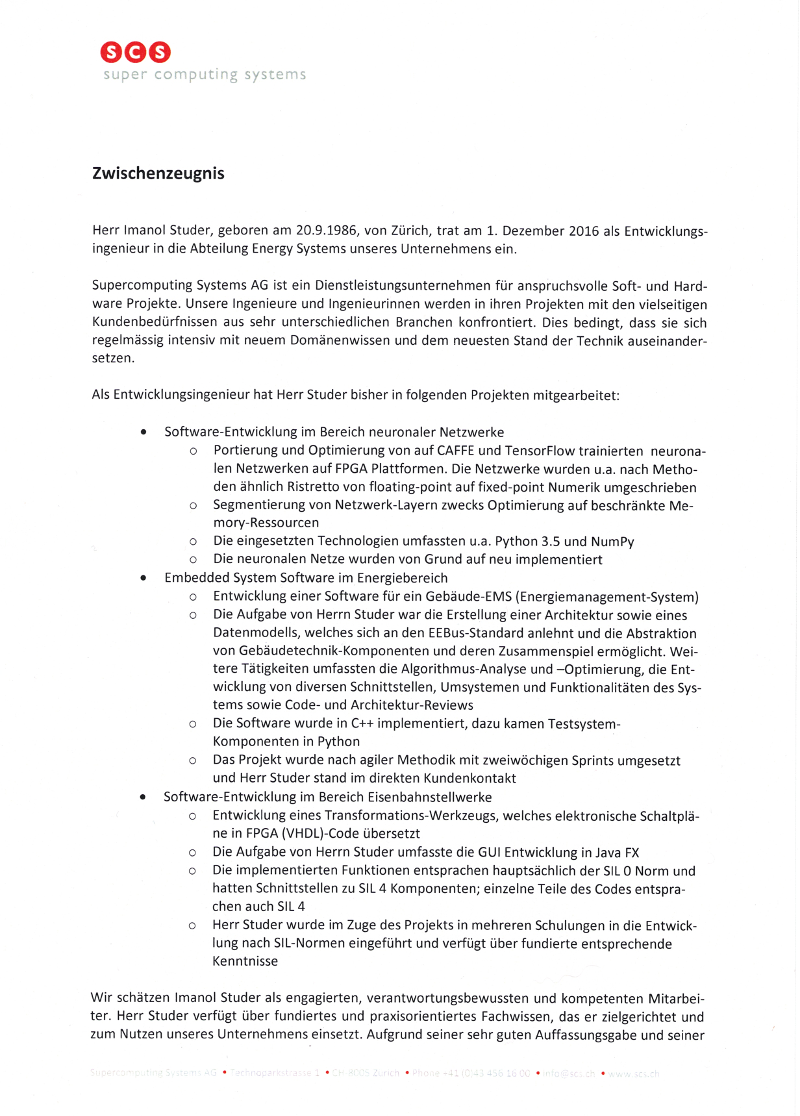
\includegraphics[width=\textwidth]{pictures/bachelor/page0.png}
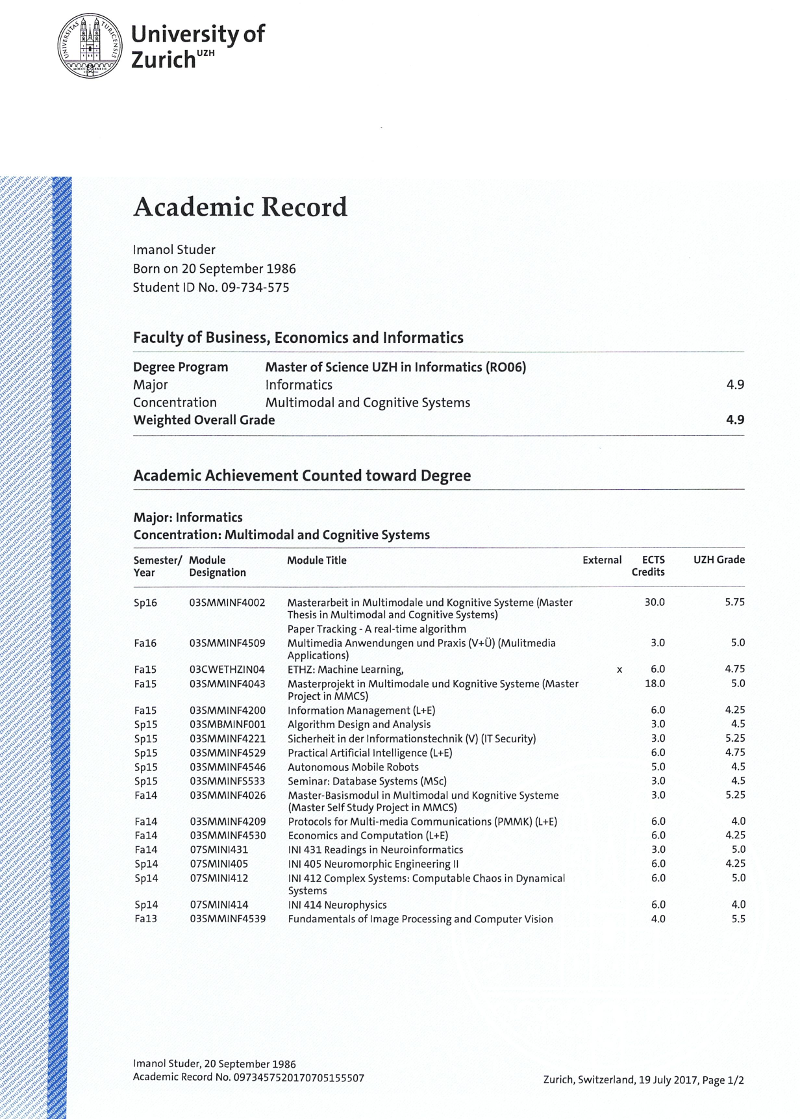
\includegraphics[width=\textwidth]{pictures/bachelor/page1.png}
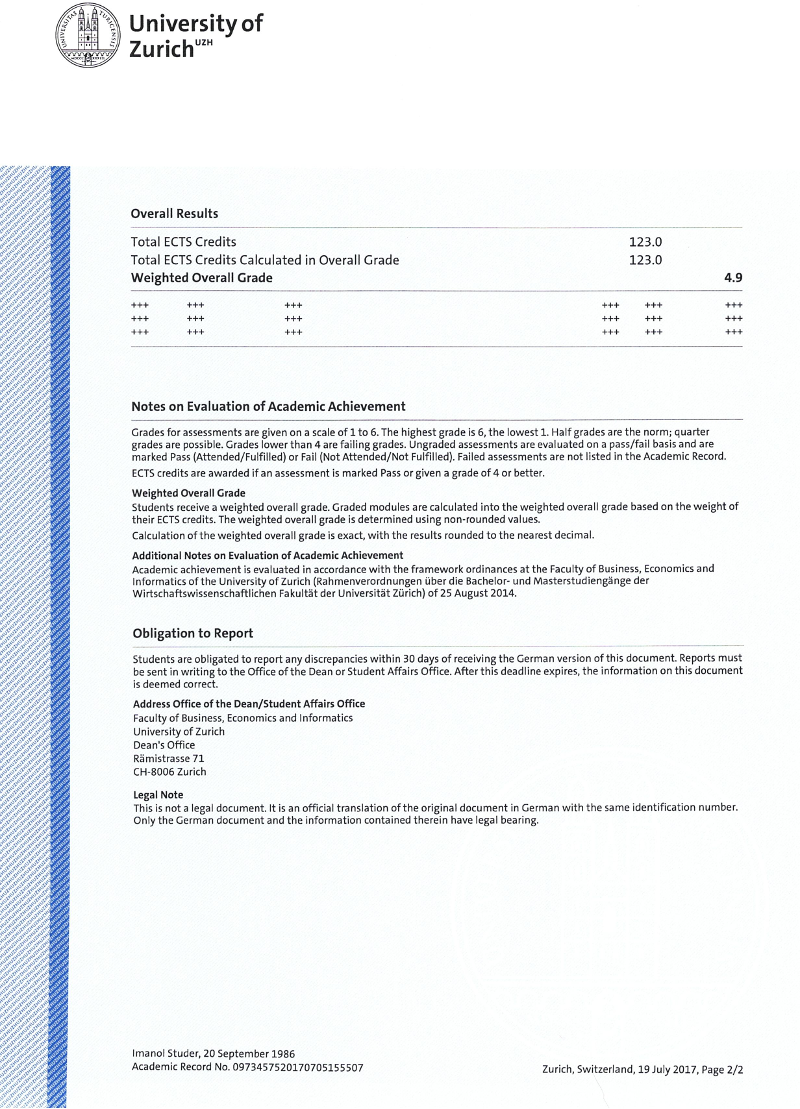
\includegraphics[width=\textwidth]{pictures/bachelor/page2.png}
\includegraphics[width=\textwidth]{pictures/bachelor/page3.png}

\restoregeometry